\section{Saules apstarojums}

Lielākā daļa Saules emitētās enerģijas tiek saražota kodolreakcijās fotosfērā. 
Kopējais saules apstarojums (\textit{Total Solar Irradiance} -- TSI) raksturo Saules starojuma absolūto intensitāti -- enerģiju uz virsmas perpendikulāri starojuma izplatīšanas virzienam 1 AU attālumā no Saules, integrētu visā saules enerģijas diskā un visā saules enerģijas spektrā. TSI vērtībai novērojama aptuveni 11 gadus ilga periodiska variācija, kas korelē ar saules plankumu skaitli (\ref{fig:TSI_misijas}. att.) -- par Saules plankumu sauc magnētiskās plūsmas koncentrāciju bipolāros klāsteros vai grupās izraisītos tumšos plankums uz Saules fotosfēras; Saules plankumu skaitlis ir atkarīgs no individuālu Saules plankumu un to grupu skaita \cite{ThermalProcesses}.

TSI norāda uz solārās radiācijas izmaiņām, kas ietekmē saņemto solārās enerģijas apjomu, kas nonāk Zemes atmosfēras augšējos slāņos. Papildus ir noderīgi zināt Saules emitētā starojuma spektrālo sadalījumu (\textit{Spectral Solar Irradiance} -- SSI) -- \ref{fig:SSI}. att. redzams, ka aptuveni puse starojuma tiek saņemta salīdzinoši mazu viļņu garumu - 380 -- 780 nm diapazonā.
 % kas padara iespējumu no tā iegūt enerģiju ar saules paneļu paņēmienu pēc formulām \ref{eq:proof}. 
% kādēļ tieši šis diapazons?
% atradu cik šī diapazona laukums ir procenti no visa laukuma un negribēju rēķināt citu
% mazs viļņu garums, tātad ar lielu frekvenci, tātad daudz enerģijas
% \begin{equation}
% \label{eq:proof}
% \nu \uparrow = \frac{c}{\lambda \downarrow} \qquad E \uparrow = h \nu \uparrow 
% \end{equation}

TSI novērojumi no kosmosa tiek veikti kopš 1978. gada (skat. tab. \ref{tab:radiometeri}.) un instrumentu specifikas dēļ iegūtas dažādas absolūtās vērtības, tāpēc šī fizikālā lieluma tikai daļēji pārkājušos novērojumu laikrindu apvienošana kompozītā ir gan zinātnisks, gan statistisks izaicinājums un neviens kompozīts (piemēram, PMOD, ACRIM, IRBM) līdz šim nav guvis konsensu solārā apstarojuma pētnieku kopienā (skat. att. \ref{fig:TSI_misijas}.).

\begin{figure}[h]
    \centering
    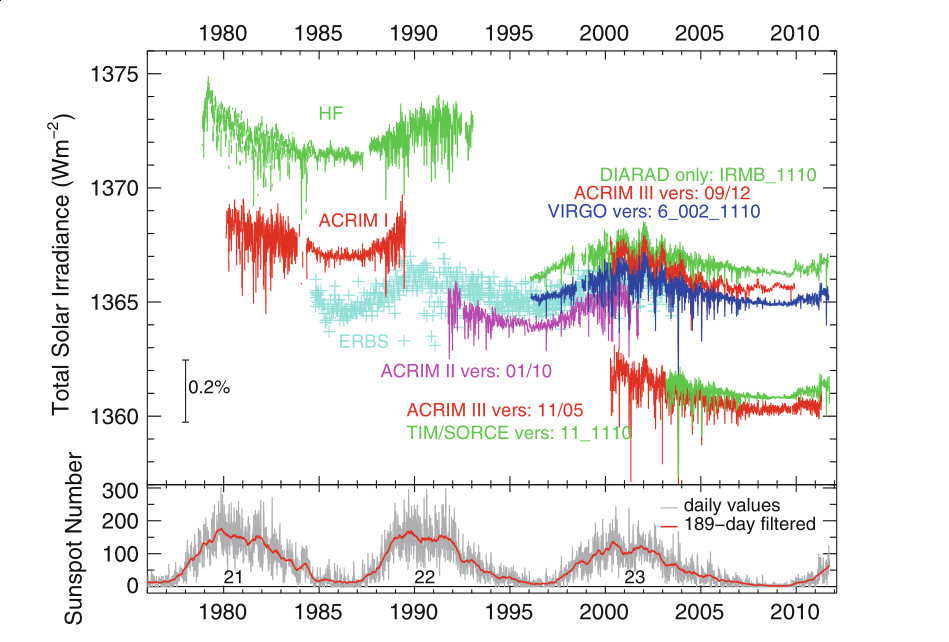
\includegraphics[width=\linewidth]{figures/misc/TSI_misijas.png}
    \caption{Salīdzinājums dienā vidējotiem saules kopējā apstarojuma datiem no dažādām kosmiskajām misijām un Saules plankuma skaitlis, lai ilustrētu solārās aktivitātes variabilitāti trīs ciklos \cite{Frohlich2012}.}
    \label{fig:TSI_misijas}
\end{figure}

\begin{table}[h]
    \caption{TSI mērījumu vēsture} % uzrakstīt kādu absolūto TSI izmērīja vai norādīt uz grafiku?
    \begin{center}
    \begin{tabular}{| r | c | l |}
    \hline
    Radiometrs & Misija & Darbības laiks \\ \hline
    Hickey-Frieden & NIMBUS-7 & 1978--1992  \\ \hline
	ACRIM I & Solārā Maksimuma Misija (SMM) & 1980--1989 \\ \hline
	ACRIM  & Zemes Radiācijas Budžeta Satelīts (ERBS) & 1984--2003 \\ \hline
	ACRIM II & Augšējās Atmosfēras Izpētes Satelīts (UARS) & 1991--2001 \\ \hline
	VIRGO & Solārā un Heliosfēras observatorija (SOHO)& 1996--pašlaik \\ \hline
	ACRIM III & ACRIMSAT  & 2000--pašlaik \\ \hline
	TIM & Saules Radiācijas un Klimata Eksperiments (SORCE) & 2003--pašlaik\\ \hline
    \end{tabular}
    \end{center}
    \label{tab:radiometeri}
\end{table}

Par labāko Saules apstarojuma mērījumu reprezentāciju tiek uzskatīti TIM instrumenta dati mēraparāta uzbūves -- atšķirībā no citiem radiometriem TIM precizitātes apertūra atrodas tuvu dobumam un redzeslauku bloķējošā apertūra ir pie instrumenta ieejas -- un augstās precizitātes -- nenoteiktība tiek novērtēta esam mazāk nekā $0.014\textrm{Wm}^{-2}\textrm{yr}^{-1}$ un precizitāte ar $0.48\textrm{Wm}^{-2}$ \cite{TSIdata} -- dēļ, tāpēc šajā darbā grafiki balstās uz šiem mērījumiem, pēc kuriem absolūtā kopējā saules apstarojuma vērtība ir $1360.8 \pm 0.5 \textrm{Wm}^{-2}$~\cite{Frohlich2012}.

\begin{figure}[h]
    \centering
    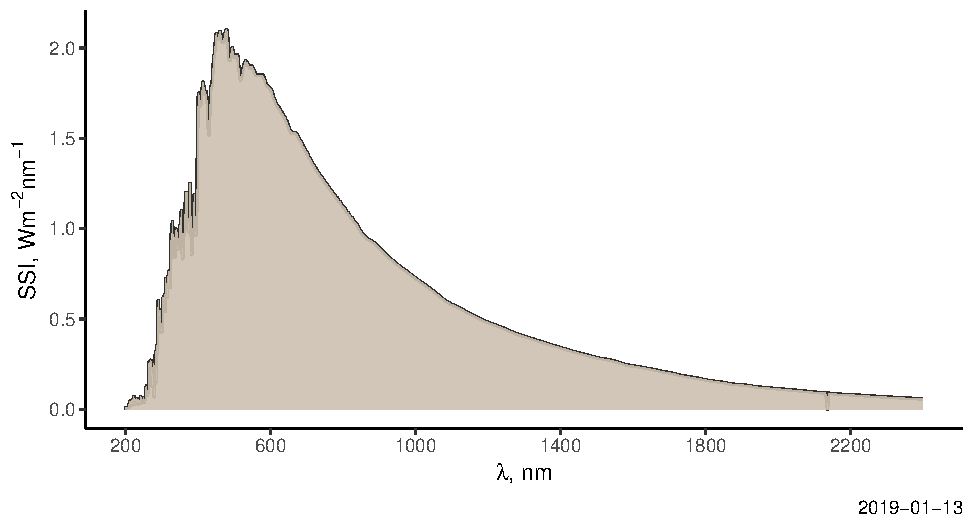
\includegraphics[width=\linewidth]{figures/misc/SSI.pdf}
    \caption{SSI 1AU attālumā (24 h vidējā vērtība) \cite{SSIdata}.}
    \label{fig:SSI}
\end{figure}

\begin{figure}[h]
    \centering
    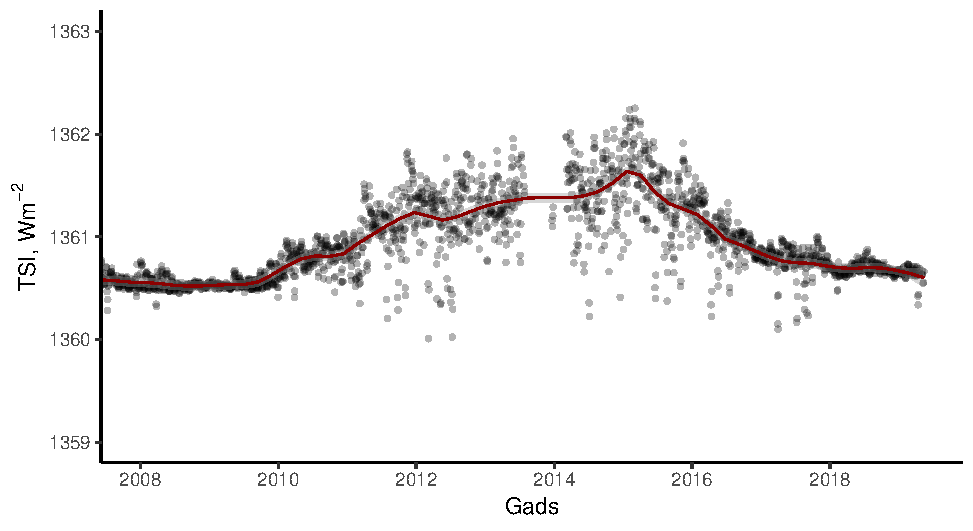
\includegraphics[width=\linewidth]{figures/misc/TSI_8-19.pdf}
    \caption{TSI 24. saules ciklā 1 AU attālumā (24 h vidējā vērtība)\cite{TSIdata}.}
    \label{fig:TSI1}
\end{figure}

\begin{figure}[h]
    \centering
    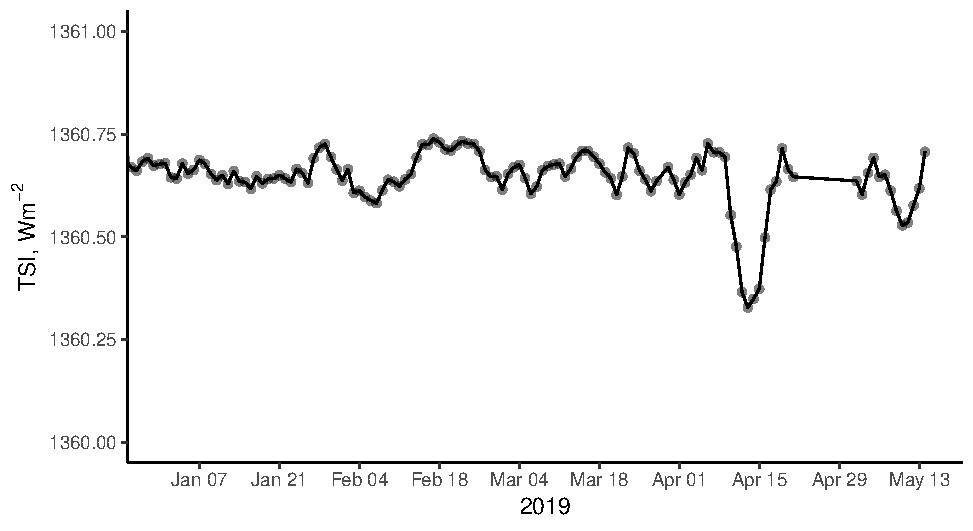
\includegraphics[width=\linewidth]{figures/misc/TSI.pdf}
    \caption{TSI izmaiņas solāro paneļu datu ieguves laikā 1 AU attālumā (24 h vidējā vērtība)\cite{TSIdata}.}
    \label{fig:TSI2}
\end{figure}
